\documentclass[
size=17pt,
paper=smartboard,
mode=present,
display=slidesnotes,
style=sailor,
nopagebreaks,
blackslide,
fleqn]{powerdot}
 %wj capsules prettybox
 %mode = handout or present

\usepackage{amsmath,graphicx,color,amsfonts}
\usepackage[brazilian]{babel}
\usepackage[utf8]{inputenc}

\pdsetup{
   lf = {EC01045 PDS},
   rf = {Sinais e Sistemas Discretos},palette ={Sea},randomdots={false}
}


%opening
\title{\Large EC01045 -- Processamento Digital de Sinais\\ \vspace{1cm}Sinais e Sistemas Discretos}
\author{Ronaldo de Freitas Zampolo\\FCT-ITEC-UFPA}
\date{ }

\begin{document}
   \maketitle[randomdots={false}]
   \begin{slide}{Agenda}
      \tableofcontents[content=sections]
   \end{slide}

% \section[slide=false]{Agenda}
% \begin{slide}{T\'opicos do capítulo}
% \scriptsize{
% \begin{itemize}
%   \item Sinais discretos
%   \item Sistemas discretos
%   \item Sistemas lineares e invariantes
%   \item Propriedades dos sistemas lineares e invariantes
%   \item Equações de diferença
%   \item Representação no domínio da frequência
%   \item Representação de sequências por Transformada de Fourier
%   \item Propriedades da Transformada de Fourier
%   \item Teoremas da Transformada de Fourier
%   \item Sinais discretos aleatórios
% \end{itemize}}
% \end{slide}

% Continuar convolução
\section[slide=false]{Sistemas lineares e invariantes} 
\begin{slide}{Convolução}
   \begin{equation*}
      y[n]=x[n]*h[n]=\sum_{k=-\infty}^{\infty}x[k]h[n-k]
   \end{equation*}
   \begin{center}
      \onslide*{1}{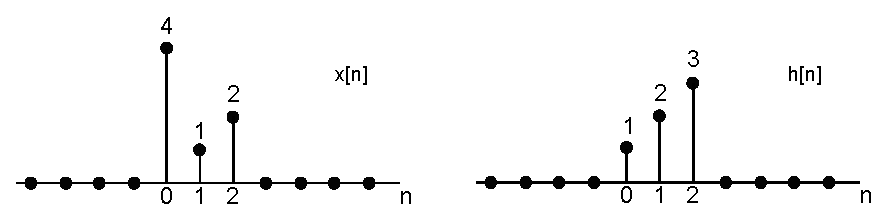
\includegraphics[width=\textwidth]{figs/doissinais.eps}}
      \onslide*{2}{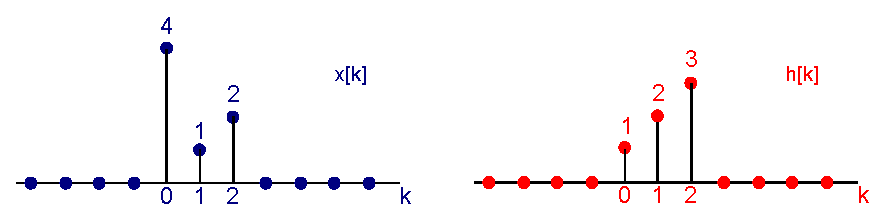
\includegraphics[width=\textwidth]{figs/doissinais2.eps}}
      \onslide*{3}{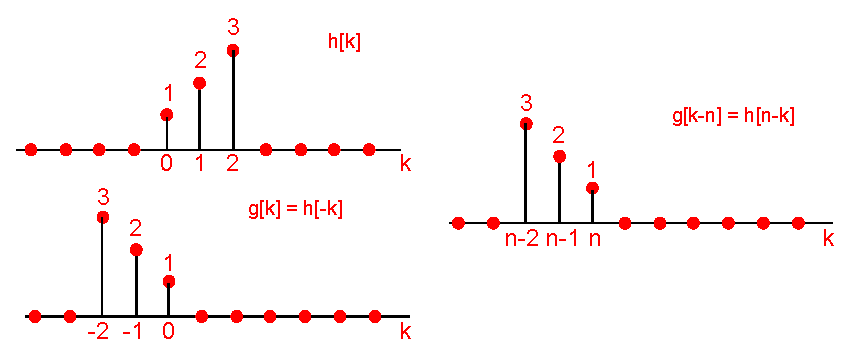
\includegraphics[width=\textwidth]{figs/hs.eps}}
      \onslide*{4}{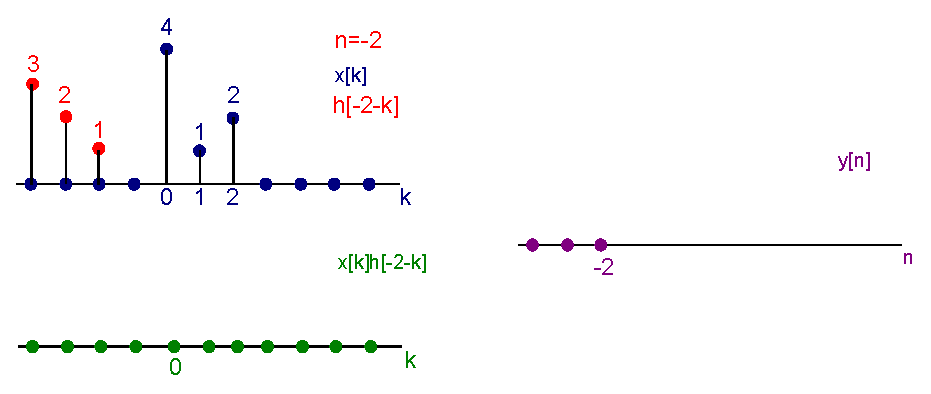
\includegraphics[width=\textwidth]{figs/step1.eps}}
      \onslide*{5}{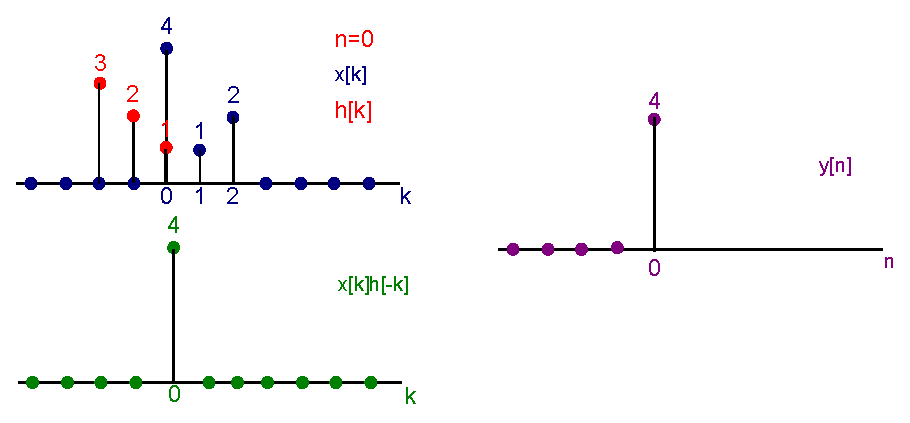
\includegraphics[width=\textwidth]{figs/step2.eps}}
      \onslide*{6}{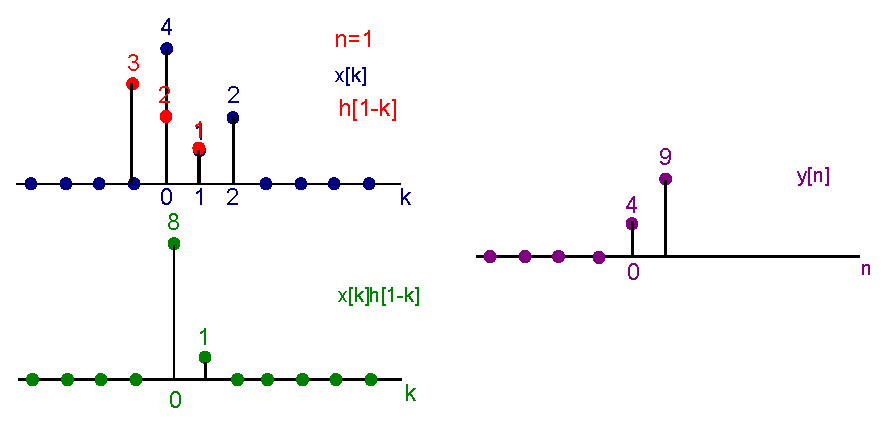
\includegraphics[width=\textwidth]{figs/step3.eps}}
      \onslide*{7}{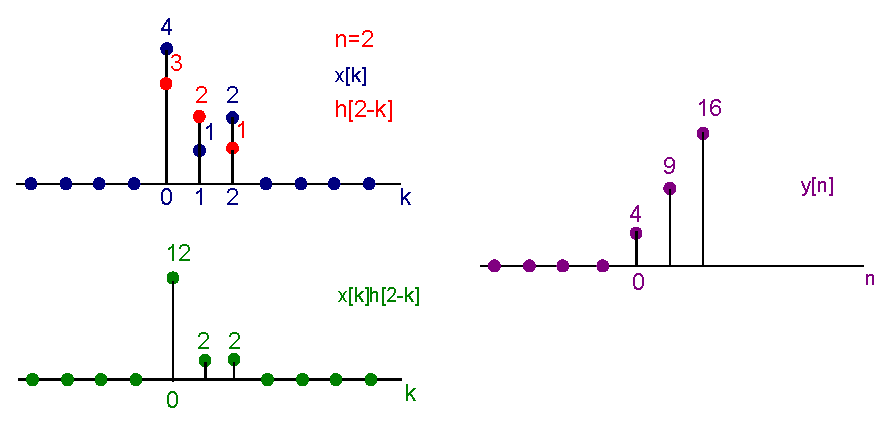
\includegraphics[width=\textwidth]{figs/step4.eps}}
      \onslide*{8}{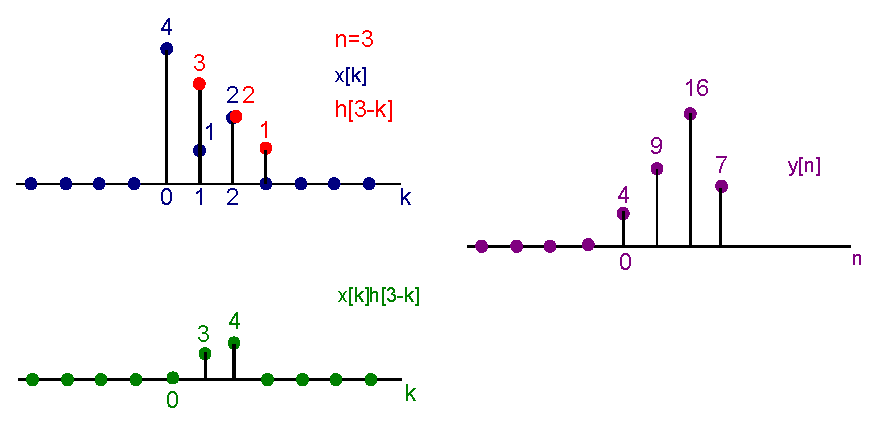
\includegraphics[width=\textwidth]{figs/step5.eps}}
      \onslide*{9}{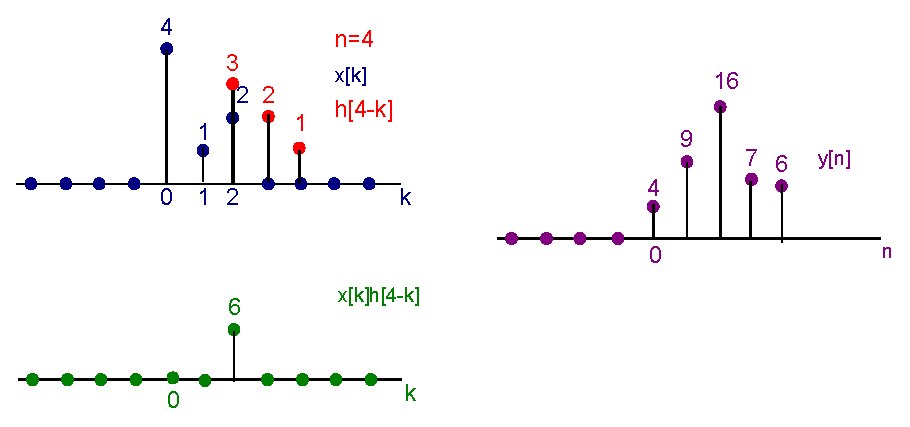
\includegraphics[width=\textwidth]{figs/step6.eps}}
      \onslide*{10}{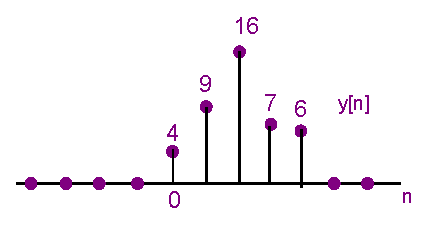
\includegraphics[width=0.7\textwidth]{figs/y.eps}}
   \end{center}
\end{slide}

\section[slide=false]{Propriedades dos sistemas LI}
\begin{slide}{Comutatividade}
   \begin{itemize}
    \item $x[n]\ast h[n] = h[n]\ast x[n]$
    \item Sistemas em cascata:
    \setlength{\unitlength}{1cm}
    \begin{center}
    \begin{picture}(7,3.5)
      \thicklines
      \put( 0, 0.5 ) {\vector(1,0){1}}
      \put( 1, 0 ) {\framebox( 5, 1){$h_1[n]\ast h_2[n]$}}
      %\put( 3, 0.5 ) {\vector(1,0){1}}
      %\put( 4, 0 ) {\framebox( 2, 1){$h_2[n]$}}
      \put( 6, 0.5 ) {\vector(1,0){1}}
      
      \put(0.3,0){$x$}
      \put(6.3,0){$y$}
      
      \put( 0, 1.75 ) {\vector(1,0){1}}
      \put( 1, 1.25 ) {\framebox( 2, 1){$h_2[n]$}}
      \put( 3, 1.75 ) {\vector(1,0){1}}
      \put( 4, 1.25 ) {\framebox( 2, 1){$h_1[n]$}}
      \put( 6, 1.75 ) {\vector(1,0){1}}
      
      \put(0.3,1.25){$x$}
      \put(6.3,1.25){$y$}
      
      \put( 0, 3 ) {\vector(1,0){1}}
      \put( 1, 2.5 ) {\framebox( 2, 1){$h_1[n]$}}
      \put( 3, 3 ) {\vector(1,0){1}}
      \put( 4, 2.5) {\framebox( 2, 1){$h_2[n]$}}
      \put( 6, 3 ) {\vector(1,0){1}}
      
      \put(0.3,2.5){$x$}
      \put(6.3,2.5){$y$}
      
    \end{picture}
    \end{center}
   \end{itemize}
\end{slide}


\begin{slide}{Distributividade}
   \begin{itemize}
    \item $x[n]\ast\left ( h_1[n]+h_2[n]\right ) = x[n]\ast h_1[n]+ x[n]\ast h_2[n]$
    \item Sistemas em paralelo:
    \setlength{\unitlength}{1cm}
    \begin{center}
    \begin{picture}(7,3.5)
      \thicklines
      \put( 0, 0.5 ) {\vector(1,0){1}}
      \put( 1, 0 ) {\framebox( 5, 1){$h_1[n]+ h_2[n]$}}
      \put( 6, 0.5 ) {\vector(1,0){1}}
      
      \put(0.3,0){$x$}
      \put(6.3,0){$y$}
      %------------------------
      \put(2.5, 1.25){\framebox(2,1){$h_2[n]$}}
      \put(2.5, 2.5){\framebox(2,1){$h_1[n]$}}
      \put(1.5, 1.75){\vector(1,0){1}}
      \put(1.5, 3){\vector(1,0){1}}
      \put(1.5, 3){\line(0,-1){1.25}}
      \put(4.5, 1.75){\line(1,0){1}}
      \put(4.5, 3){\line(1,0){1}}
      
      \put(5.5,2.375){\circle{0.5}}
      \put(5.75,2.375){\vector(1,0){1}}
      \put(0.5,2.375){\vector(1,0){1}}
      \put(5.5,1.75){\vector(0,1){0.375}}
      \put(5.5,3){\vector(0,-1){0.375}}
      \put(5.35,2.275){+}
      
      \put(0.8,1.875){$x$}
      \put(6.05,1.875){$y$}
    \end{picture}
    \end{center}
   \end{itemize}
\end{slide}

\begin{slide}{Causalidade}
   \begin{itemize}
      \item Causalidade: \\
            Um sistema LI é causal se\begin{equation*} h[n] = 0, \quad n<0 \end{equation*}
            Por que?
   \end{itemize}
\end{slide}

\begin{slide}{Estabilidade 1}
   \begin{itemize}
    \item Um sistema LI é estável se
    \begin{equation*}
        S = \sum_{n=-\infty}^{\infty}|h[n]|<\infty
    \end{equation*}
    
    A resposta do sistema ao impulso é \textcolor{red}{absolutamente somável} (condição suficiente
    e necessária para estabilidade).\pause
    \begin{align*}
       |y[n]|&=\left | \sum_{k=-\infty}^{\infty} h[k]x[n-k]\right |\\
             &\leq \sum_{k=-\infty}^{\infty} |h[k]||x[n-k]|
    \end{align*}
    %Se $x[n]\leq B_x < \infty$, então $|y[n]|\leq B_x\sum_{k=-\infty}^{\infty} |h[k]|$
   \end{itemize}
\end{slide}

\begin{slide}{Estabilidade 2}
   %\begin{itemize}
    %\item 
    Como $|x[n]|\leq B_x < \infty$ (a entrada é limitada), então 
    \begin{equation*}|y[n]|\leq \sum_{k=-\infty}^{\infty} |h[k]||x[n-k]|\leq B_x\sum_{k=-\infty}^{\infty} |h[k]|\end{equation*}\pause
    
    Logo, para que a saída seja limitada $|y[n]|\leq B_y < \infty$,
    \begin{align*}|y[n]|&\leq B_x\sum_{k=-\infty}^{\infty} |h[k]| < \infty\\
                        &\Rightarrow \boxed{\sum_{k=-\infty}^{\infty} |h[k]| < \infty}
    \end{align*}
   %\end{itemize}
\end{slide}

% \section[slide=false]{Equações de diferenças}
% \begin{slide}{Definições 1}
%    \begin{itemize}
%     \item Equação de diferenças de $N$-ésima ordem e coeficientes constantes:
%     \begin{equation*}
%        \sum_{ i = 0 }^{ N } a_i y[ n - i ]=\sum_{ \ell = 0 }^{ M } b_\ell x[ n - \ell ],
%     \end{equation*}
%     onde $x[n]$ e $y[n]$ são entrada e saída do sistema.\pause
%     \item Exemplo 01: Acumulador
%     \begin{equation*}
%        \begin{split}
%          y[n] &= \sum_{ k = -\infty}^{n} x[k]\\
%               &= y[n-1] + x[n]
%        \end{split}
%    \end{equation*}
%    \end{itemize}
% \end{slide}
% 
% \begin{slide}{Definições 2}
%    \begin{itemize}
%     \item Exemplo 02: Média móvel
%     \begin{align*}
%        %\begin{split}
%          y[n] &= \frac{1}{M_2+1}\sum_{ k = 0}^{M_2} x[n-k]\\
%          h[n] &= \frac{1}{M_2+1}\left ( u[n] - u[n-M_2-1] \right )\\
%               &= \frac{1}{M_2+1}\left ( \delta[n] - \delta[n-M_2-1] \right )\ast u[n]
%        %\end{split}
%     \end{align*}
%    \end{itemize}
% \end{slide}
% 
% 
% \begin{slide}{Resolução}
%    \begin{itemize}
%       \item 
% %       $y[n] = ay[n-1]+x[n]$
% %       \begin{itemize}
% %          \item $x[n]=K\delta[n]$
% %          \item $y[-1]=c$
% %          \item Para $n \geq 0$: $y[n]=a^{n+1}c+a^{n}K$
% %          \item Para $n \leq -2$: $y[n]=a^{n+1}c$
% %          \item $y[n]=a^{n+1}c+a^{n}Ku[n], \quad \quad \forall n$
% %       \end{itemize}
% %      \item $y[n]=y_p[n]+y_h[n]$
% %      \begin{itemize}
% %          \item Solução particular: $y_p[n]$
% %          \item Solução homogênea ($x[n]=0$): $y_h[n]$
% %       \end{itemize}
% %       \item Analise o sistema quanto à \textcolor{red}{linearidade}, \textcolor{red}{causalidade}, e \textcolor{red}{invariância}.
%    \end{itemize}
% \end{slide}
% 
% \section[slide=false]{Representação em frequência}
%  \begin{slide}{Representação em frequência}
% \begin{itemize}
%  \item Funções exponenciais complexas como ``auto-funções'' de um sistema LI
%  %\footnotesize{
%  \begin{align*}
%    x[n]&=e^{j\omega n}\\
%    y[n]&=\sum_{k=-\infty}^{\infty}h[k]e^{j\omega (n-k)}\\
%        &=e^{j\omega n}\left [\sum_{k=-\infty}^{\infty}h[k]e^{-j\omega k} \right ]\\
%        &= H(e^{j\omega})e^{j\omega n}
%  \end{align*}%}
%  $H(e^{j\omega})$: \textcolor{red}{resposta em frequência do sistema.}
% \end{itemize}
% \end{slide}
% 
% \begin{slide}{Representação em frequência}
%  \begin{itemize}
%   \item Exemplos:
%   \begin{itemize}
%      \item Ache a $H(e^{j\omega})$ do sistema $y[n]=x[n-n_d]$.
%      \item Ache a resposta do sistema anterior para \begin{equation*}
%                                                      x[n]=\sum_k \alpha_k e^{j\omega_k n}.
%                                                     \end{equation*}
%      \item Calcule $y[n]$ em função de $H(e^{j\omega})$ de um sistema qualquer, dado $x[n]=A\cos(\omega_o n+\phi)$.
%      \item Mostre que $H(e^{j\omega})$  periódico em $2\pi$.
%   \end{itemize}
%  \end{itemize}
% \end{slide}
% 
% \section[slide=false]{Transformada de Fourier}
% \begin{slide}{Transformada de Fourier}
%  \begin{itemize}
%   \item Defini\c c\~oes
%      \begin{equation*} X(e^{j\omega})=\sum_{n=-\infty}^{\infty} x[n]e^{-j\omega n}  \end{equation*}
%      \begin{equation*} x[n]=\frac{1}{2\pi}\int_{-\pi}^{\pi} X(e^{j\omega})e^{j\omega n} d\omega \end{equation*}
%    \item Forma retangular: $X(e^{j\omega}) = X_R(e^{j\omega}) + j X_I(e^{j\omega})$
%    \item Forma polar: $X(e^{j\omega}) = |X(e^{j\omega})|e^{j\angle X(e^{j\omega})}$
%  \end{itemize}
% \end{slide}
% 
% \begin{slide}{Transformada de Fourier}
%  \begin{itemize}
%   \item Prova da transformada inversa
%      \begin{align*} x[n]&= \frac{1}{2\pi}\int_{-\pi}^{\pi} X(e^{j\omega})e^{j\omega n} d\omega\\
%                        &= \frac{1}{2\pi}\int_{-\pi}^{\pi} \left ( \sum_{m=-\infty}^{\infty} x[m]e^{-j\omega m}\right )e^{j\omega n} d\omega\\
%                        & = \sum_{m=-\infty}^{\infty}x[m]\left ( \frac{1}{2\pi} \int_{-\pi}^{\pi} e^{j\omega(n-m)}d\omega \right ) \\   
%                        & = \sum_{m=-\infty}^{\infty}x[m] \delta[n-m] = x[n]\end{align*}
%   \end{itemize}
% \end{slide}
% 
% \begin{slide}{Exemplos}
% Calcule a resposta em frequência dos sistemas LI abaixo representados:
% \begin{enumerate}
%    \item $h_1[n] = a^nu[n], \quad |a|<1$
%    \item $h_2[n] = a^{|n|}, \quad |a|<1$
%    \item $h_3[n] = \begin{cases} 1,& |n|\leq N_1\\0,&|n|> N_1\end{cases}$
% \end{enumerate}
% \end{slide}
% 
% \begin{note}{Exercícios}
% Trace os gráficos de magnitude e fase das transformadas calculadas para: 
% \begin{enumerate}
%    \item $a = 0,9$
%    \item $a = -0,9$
%    \item $N_1 = 3$
%    \item $N_1 = 10$
% \end{enumerate}
% Qual o comportamento esperado da transformada de Fourier de $h_3[n]$ quando $N_1\rightarrow 0$ ?
% \end{note}
% 
% \section[slide=false]{Propriedades da Transf. de Fourier}
% \begin{slide}{Propriedades da Transf. de Fourier}
% \begin{itemize}
%    \item Sequ\^encias  sim\'etrica e anti-sim\'etrica conjugadas
%    \begin{align*}
%       x[n] &= x_e[n]+x_o[n]\\
%       x_e[n] &= \frac{1}{2} \left \{ x[n] + x^*[-n] \right \} = x_e^*[-n]\\
%       x_o[n] &= \frac{1}{2} \left \{ x[n] - x^*[-n] \right \} = -x_o^*[-n]
%    \end{align*} 
% \end{itemize}
% \end{slide}
% 
% \begin{slide}{Propriedades da Transf. de Fourier}
% \begin{itemize}
%    \item Sequ\^encias  sim\'etrica e anti-sim\'etrica conjugadas
% \begin{itemize}
%    \item $x^*[n]\stackrel{F}{\leftrightarrow} X^*(e^{-j\omega})$
%    \item $x^*[-n]\stackrel{F}{\leftrightarrow} X^*(e^{j\omega})$
%    \item $\Re\{x[n]\} \stackrel{F}{\leftrightarrow} X_e(e^{j\omega})$
%    \item $j\Im\{x[n]\} \stackrel{F}{\leftrightarrow} X_o(e^{j\omega})$
%    \item $x_e[n] \stackrel{F}{\leftrightarrow} X_R(e^{j\omega}) = \Re\{X(e^{j\omega})\}$
%    \item $x_o[n] \stackrel{F}{\leftrightarrow} jX_I(e^{j\omega}) = j\Im\{X(e^{j\omega})\}$
% \end{itemize}
% \end{itemize}
% \end{slide}
% 
% 
% \begin{slide}{Propriedades da Transf. de Fourier}
% \begin{itemize}
%    \item Para $x[n]$ real
%    \begin{itemize}
%       \item $ X(e^{j\omega}) = X^*(e^{-j\omega})$
%       \item $ X_R(e^{j\omega}) = X_R(e^{-j\omega})$
%       \item $ X_I(e^{j\omega}) = -X_I(e^{-j\omega})$
%       \item $ |X(e^{j\omega})| = |X(e^{-j\omega})|$
%       \item $ \angle X(e^{j\omega}) = -\angle X(e^{-j\omega})$
%       \item $ x_o[n] \stackrel{F}{\leftrightarrow} X_R(e^{j\omega})$
%       \item $ x_e[n] \stackrel{F}{\leftrightarrow} jX_I(e^{j\omega})$
%    \end{itemize}
% \end{itemize}
% \end{slide}
% 
% \section[slide=false]{Teoremas da Transf. de Fourier}
% \begin{slide}{Teoremas da Trans. de Fourier}
% \center{
% \small{\begin{tabular}{l|l}
% \hline
% Sequência & Transformada de Fourier \\
% \hline
% $x[n]$     &   $X(e^{j\omega})$ \\
% $y[n]$     &   $Y(e^{j\omega})$\\
% \hline
% 1. $ax[n]+by[n]$ & $aX(e^{j\omega})+bY(e^{j\omega})$\\
% 2. $x[n-n_d]$ & $e^{-j\omega n_d}X(e^{j\omega})$ \\
% 3. $e^{j\omega_o n}x[n]$ & $X(e^{j(\omega-\omega_o)})$\\
% 4. $x[-n]$ & $X(e^{-j\omega})$\\
%            & $X^*(e^{j\omega})$ se $x[n]$ for real\\
% 5. $nx[n]$ & $j\frac{dX(e^{j\omega})}{d\omega}$\\
% 6. $x[n]*y[n]$ & $X(e^{j\omega})Y(e^{j\omega})$\\
% 7. $x[n]y[n]$ & $\frac{1}{2\pi}\int_{-\pi}^{\pi} X(e^{j\theta})Y(e^{j(\omega-\theta)})d\theta$\\
% \hline
% \multicolumn{2}{l}{8. $\sum_{n=-\infty}^{\infty}|x[n]|^2=\frac{1}{2\pi}\int_{-\pi}^{\pi}|X(e^{j\omega})|^2d\omega$}\\
% \multicolumn{2}{l}{9. $\sum_{n=-\infty}^{\infty}x[n]y^*[n]=\frac{1}{2\pi}\int_{-\pi}^{\pi}X(e^{j\omega})Y^*(e^{j\omega})d\omega$}\\
% \hline
% \end{tabular}}}
% \end{slide}
% 
% \begin{note}{Exercícios}
% \begin{enumerate}
%    \item Deduza cada uma das propriedades da transformada de Fourier.
%    \item Prove cada um dos teoremas da transformada de Fourier. 
% \end{enumerate}
% 
% \end{note}
% 
% 
% \section[slide=false]{Sinais discretos aleatórios}
% \begin{slide}{Sinais determinísticos}
% \begin{itemize}
%    \item Definidos unicamente
%    \begin{itemize}
%       \item Express\~ao matem\'atica
%       \item Tabela
%       \item Algum tipo de regra
%    \end{itemize}
%    
% \end{itemize}
% \end{slide}
% 
% \begin{slide}{Sinais aleatórios}
% \begin{itemize}
%    \item Processos aleat\'orios $\times$ Vari\'aveis aleat\'orias
%    \item Processo estacion\'ario
%    \begin{itemize}
%       \item Sentido estrito
%       \item Sentido amplo
%       \begin{align*}
%          m_x[n] &= E\{x[n]\} = k\\
%          \phi_{xx}[n,n+m] &= E\{x[n]x[n+m]\}= \phi_{xx}[m]
%       \end{align*}
%    \end{itemize}
% \end{itemize}
% \end{slide}
% 
% \begin{slide}{Entrada estacionária (EE) -- média}
% \begin{itemize}
%    \item Entrada estacion\'aria $\Rightarrow$ Sa\'ida estacion\'aria
%    \item M\'edia
%    \begin{align*}
%       m_y[n] &= E\{y[n]\}\\
%              &= E\left \{\sum_{k=-\infty}^{\infty} h[n-k] x[k]\right \}\\
%              &= \sum_{k=-\infty}^{\infty} h[n-k] E\{x[k]\}\\
%              &= m_x H\left (e^{j0}\right )
%    \end{align*}
% \end{itemize}
% \end{slide}
% 
% \begin{slide}{EE -- autocorrela\c c\~ao}
%    \scriptsize{
%    \begin{align*}
%       \phi_{yy}[n,n+m] &= E\{y[n]y[n+m]\}\\
%              &= E\left\{\sum_{k=-\infty}^{\infty} h[k] x[n-k]\sum_{r=-\infty}^{\infty} h[r] x[n+m-r]\right\}\\
%              &= \sum_{k=-\infty}^{\infty} \sum_{r=-\infty}^{\infty} h[k]h[r] E\{x[n-k]x[n+m-r]\}\\
%              &= \sum_{k=-\infty}^{\infty} \sum_{r=-\infty}^{\infty} h[k]h[r] \phi_{xx}[m-r+k]\\
%              &= \sum_{k=-\infty}^{\infty} \sum_{l=-\infty}^{\infty} h[k]h[l+k] \phi_{xx}[m-l]\\
%              &= \sum_{l=-\infty}^{\infty} \phi_{xx}[m-l]\sum_{k=-\infty}^{\infty} h[k]h[l+k] \\
%              &= \sum_{l=-\infty}^{\infty} \phi_{xx}[m-l] c_{hh}[l] \\
%              &= \phi_{xx}[m]*c_{hh}[m]\\
%     %c_{hh}[n]&= h[n]*h[-n]  \quad\text{autocorr. determin\'istica}
%    \end{align*}}
% \end{slide}
% 
% 
% \begin{slide}{EE -- Densidade Espectral de Pot\^encia}
% \begin{align*}
%    \Phi_{yy}(e^{j\omega}) &= \sum_{m=-\infty}^{\infty}  \phi_{yy}[m]e^{-j\omega m}\\
%                           &= \sum_{m=-\infty}^{\infty}  \{\phi_{xx}[m]*c_{hh}[m]\} e^{-j\omega m}\\
%                           &= \Phi_{xx}(e^{j\omega}) C_{hh}(e^{j\omega})
% \end{align*}
% \begin{equation*}
%      \boxed{\Phi_{yy}(e^{j\omega}) = \Phi_{xx}(e^{j\omega}) |H(e^{j\omega})|^2}
%   \end{equation*}
% \end{slide}
% 
% % \begin{slide}{Sinais discretos aleat\'orios}
% % \begin{itemize}
% %    \item Densidade Espectral de Pot\^encia
% %    \begin{align*}
% %     %  \Phi_{yy}(e^{j\omega}) &= \sum_{m=-\infty}^{\infty}  \phi_{yy}[m]e^{-j\omega m}\\
% %     %                         &= \sum_{m=-\infty}^{\infty}  \{\phi_{xx}[m]*c_{hh}[m]\} e^{-j\omega m}\\
% %     %                         &= \Phi_{xx}(e^{j\omega}) C_{hh}(e^{j\omega})
% %     C_{hh}(e^{j\omega})       &= \sum_{m=-\infty}^{\infty} c[m] e^{-j\omega m} \\
% %                               &= \sum_{m=-\infty}^{\infty} \sum_{k=-\infty}^{\infty}h[k]h[m+k] e^{-j\omega m} \\
% %                               &= \sum_{k=-\infty}^{\infty} h[k]\sum_{m=-\infty}^{\infty}h[m+k] e^{-j\omega m} 
% %                               %&= H(e^{j\omega})\sum_{k=-\infty}^{\infty} h[k]e^{j\omega k} \\
% %                               %&= H(e^{j\omega})H^*(e^{j\omega})\\
% %                               %&= |H(e^{j\omega})|^2
% %    \end{align*}
% % \end{itemize}
% % \end{slide}
% % 
% % \begin{slide}{Sinais discretos aleat\'orios}
% % \begin{itemize}
% %    \item Densidade Espectral de Pot\^encia
% %    \begin{align*}
% %     %  \Phi_{yy}(e^{j\omega}) &= \sum_{m=-\infty}^{\infty}  \phi_{yy}[m]e^{-j\omega m}\\
% %     %                         &= \sum_{m=-\infty}^{\infty}  \{\phi_{xx}[m]*c_{hh}[m]\} e^{-j\omega m}\\
% %     %                         &= \Phi_{xx}(e^{j\omega}) C_{hh}(e^{j\omega})
% %     C_{hh}(e^{j\omega})       %&= \sum_{m=-\infty}^{\infty} c[m] e^{-j\omega m} \\
% %                               %&= \sum_{m=-\infty}^{\infty} \sum_{k=-\infty}^{\infty}h[k]h[m+k] e^{-j\omega m} \\
% %                               %&= \sum_{k=-\infty}^{\infty} h[k]\sum_{m=-\infty}^{\infty}h[m+k] e^{-j\omega m} 
% %                               &= H(e^{j\omega})\sum_{k=-\infty}^{\infty} h[k]e^{j\omega k} \\
% %                               &= H(e^{j\omega})H^*(e^{j\omega})\\
% %                               &= |H(e^{j\omega})|^2\\
% %     \Phi_{yy}(e^{j\omega}) &= \Phi_{xx}(e^{j\omega}) C_{hh}(e^{j\omega})
% %     %\Phi_{yy}(e^{j\omega}) &= \Phi_{xx}(e^{j\omega}) |H(e^{j\omega})|^2
% %   \end{align*}
% %      
% %   \begin{equation*}
% %      \boxed{\Phi_{yy}(e^{j\omega}) = \Phi_{xx}(e^{j\omega}) |H(e^{j\omega})|^2}
% %   \end{equation*}
% % \end{itemize}
% % \end{slide}
% 
% \begin{slide}{Sinais discretos aleat\'orios}
% \begin{itemize}
%    \item C\'alculo da pot\^encia de um sinal
%    \begin{align*}
%       E\{y^2[n]\} &= E\{y[n]y[n]\}\\
%                   &= \phi_{yy}[0]\\
%                   &= \frac{1}{2\pi}\int_{-\pi}^{\pi}\Phi_{yy}(e^{j\omega})d\omega 
%    \end{align*}
% \end{itemize}
% \end{slide}
% 
\end{document}
